\documentclass[]{beamer}
\usepackage[T1]{fontenc}
\usepackage[utf8]{inputenc}
\usepackage{lmodern}
\usepackage[italian]{babel}
\usepackage{mathrsfs}
\usepackage{cancel}

\title{Elettrostatica e condensatori}
\author{\texorpdfstring{Mattia Cozzi\newline\href{mailto:cozzimattia@gmail.com}{\texttt{cozzimattia@gmail.com}}}{Mattia Cozzi}}
\date{a.s.~2023/2024}

%\documentclass[handout]{beamer}     %usare questa classe per generare l'handout
%\usepackage{pgfpages}   %per mostrare più quadri nella stessa pagina
%\pgfpagesuselayout{4 on 1}[a4paper,border shrink=5mm,landscape]
\usetheme{Singapore}
%\useoutertheme[left]{sidebar} %elementi intorno alle diapositive
\setbeamercovered{dynamic} %modifica l'aspetto del testo grigetto delle diapositive future. Argomenti: invisible/transparent/dynamic
\usecolortheme{orchid}
%COLORE PRINCIPALE
% \definecolor{marroncino}{RGB}{156, 26, 0} % UBC Blue (primary)
% \setbeamercolor{structure}{fg=marroncino} % itemize, enumerate, etc

\theoremstyle{plain}
\newtheorem{teorema}{Teorema}

\usepackage{tikz}
\usepackage{circuitikz}

\usepackage{pgf,pgfplots,graphicx}
\usetikzlibrary{angles,quotes,arrows,shapes,decorations.markings}
\pgfplotsset{compat=1.15}
\usepgfplotslibrary{units,fillbetween} % to add units easily to axis

\newcommand{\fem}{f_{em}}

\def\angolo[#1](#2)(#3:#4:#5)% Syntax: [draw options] (center) (initial angle:final angle:radius)
    { \draw[#1] ($(#2)+({#5*cos(#3)},{#5*sin(#3)})$) arc (#3:#4:#5); }


\newcommand<>{\xxcancel}[1]{\alt#2{\xcancel{#1}\vphantom{#1}}{#1}}

\begin{document}

\begin{frame}
  \titlepage
\end{frame}





\begin{frame}
\frametitle{Contenuti}
\tableofcontents
\end{frame}


\section{Conduttori}




\begin{frame}
\frametitle{Conduttori}
Un materiale è conduttore se le cariche in eccesso possono \alert<1>{muoversi liberamente} al suo interno.{\pause}

~

Ad esempio:
\begin{itemize}
  \item solidi:
  \begin{itemize}
    \item i metalli;
    \item il carbonio in alcune configurazioni (grafite e grafene);
    \item alcuni ossidi trasparenti (come l'ossido di indio-stagno, usato nei \emph{touchscreen}.
  \end{itemize}\pause
  \item liquidi:
  \begin{itemize}
    \item metalli fusi (come $ Hg $ a $ 293 \, K $);
    \item le soluzioni elettrolitiche;
  \end{itemize}\pause
  \item gas, solo se ionizzati.
\end{itemize}
\end{frame}

\begin{frame}
\frametitle{Conduttore in equilibrio}
Consideriamo un conduttore solido in condizione di \alert{equilibrio elettrostatico}, in cui non c'è moto di cariche.\pause

~

La condizione di stasi implica che $ \sum \vec{F} = 0 $ e pertanto, poiché la definizione di campo elettrico ci dice che $ \vec{E} = \dfrac{\vec{F}}{q} $:
\begin{center}
\colorbox{blue!30}{il campo elettrico all'interno del conduttore è nullo}
\end{center}
\begin{figure}
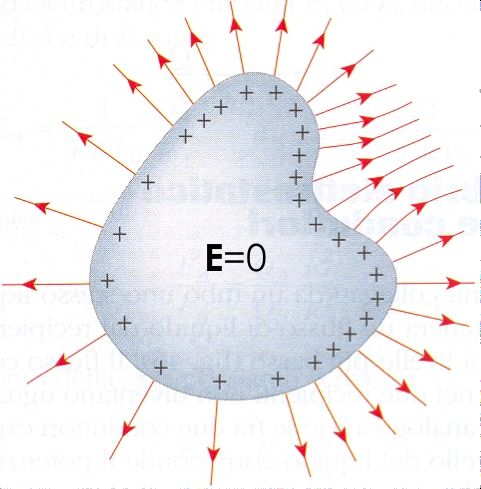
\includegraphics[width=.3\columnwidth]{img/conduttoreequilibrio.png}
\end{figure}
\end{frame}

\begin{frame}
\frametitle{Distribuzione della carica}
Se il conduttore è carico, \alert<1>{la sua carica deve necessariamente trovarsi sulla superficie esterna}, confinata in un sottile strato di spessore trascurabile\footnote{Per un metallo è nell'ordine di $ 10^{-10} \, m $.}.\pause

~

Il campo $ \vec{E} $ che il conduttore carico esercita intorno a sé è sempre \alert<2>{perpendicolare alla superficie del conduttore}: se non lo fosse, metterebbe in moto le cariche sulla superficie.\pause

~

La superficie del conduttore risulta una \alert<3>{superficie equipotenziale}.
\end{frame}


\begin{frame}
\frametitle{La densità superficiale di carica}
Se sulla superficie $ \Delta S $ di un conduttore è presente una quantità di carica $ \Delta q $, definiamo la \alert{densità superficiale di carica} come:
\begin{center}
\colorbox{blue!30}{$ \sigma = \dfrac{\Delta q}{\Delta S} $}$ ~~~~~~ \left[ \dfrac{C}{m^2} \right] $
\end{center}\pause

~

Per un conduttore sferico, il valore di $ \sigma $ è uguale in ogni punto, in altri casi dipende dalla forma della superficie.
\end{frame}


\begin{frame}
\frametitle{Esercizio}
\begin{exampleblock}{Densità superficiale di carica}
  \small{
  Un cilindro metallico isolato di raggio di base pari a $ 1,0 \, cm $ e altezza $ 30 \, cm $ è elettrizzato con una carica di $ 6,8 \, nC $.

  Calcola la densità superficiale media di carica.\hspace*{\fill}[$ 3,5 \times 10^{-7} \, C/m^2 $]}
\end{exampleblock}
\end{frame}


\begin{frame}
\frametitle{Il teorema di Coulomb}
L'intensità del campo elettrico in prossimità della superficie di un conduttore carico è data dal \alert<1>{teorema di Coulomb}:
\begin{center}
\colorbox{blue!30}{$ E = \dfrac{\sigma}{\varepsilon_0} $}
\end{center}\pause

~

Il teorema di Coulomb si dimostra a partire dal \alert<2>{teorema di Gauss per il campo elettrico}.
\end{frame}


\section{Condensatori}


\begin{frame}
\frametitle{Il condensatore piano}
\begin{columns}
\begin{column}{0.3\textwidth}
\begin{figure}
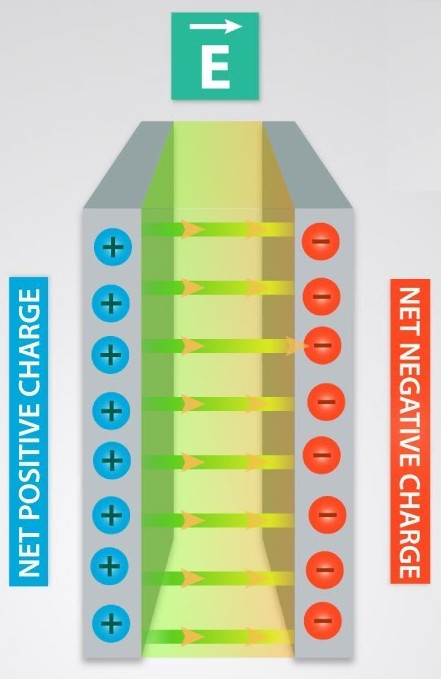
\includegraphics[width=\columnwidth]{img/condensatore.jpg}
\end{figure}
\end{column}
\begin{column}{0.7\textwidth}
Un condensatore piano è formato da due lastre metalliche parallele (armature), poste ad una piccola distanza tra loro.\pause

~

Se carichiamo un'armatura con una carica $ +Q $, sull'altra verrà indotta una carica $ -Q $.\pause

~

Tra le due armature si genera un campo elettrico pressoché uniforme di modulo:
\begin{center}
$ E = \dfrac{\sigma}{\varepsilon_0} $
\end{center}
\end{column}
\end{columns}
\end{frame}


%dimostrazione!!! però richiederebbe il campo generato da una lastra carica

\begin{frame}
\frametitle{Capacità di un condensatore piano}
Consideriamo due armature su cui è stata indotta una carica $ Q $ ($ +Q $ su quella positiva e $ -Q $ su quella negativa). Tra di esse si genera una differenza di potenziale $ \Delta V $.\pause
\begin{block}{Capacità}
La capacità di un condensatore piano è il rapporto tra la carica sulle armature e la tensione realizzata:
\begin{center}
\colorbox{blue!30}{$ C = \dfrac{Q}{\Delta V} $}
\end{center}
La capacità si misura in \emph{farad}: $ 1 \, F = 1 \, \frac{C}{V} $.
\end{block}
\end{frame}


\begin{frame}
\frametitle{Esercizio}
\begin{exampleblock}{Voltaggio di un condensatore}
  \small{
  Un condensatore di capacità $ 2,9 \, nF $ ha una carica $ Q_+ = + 7,2 \, \mu C $ sull'armatura positiva e una carica negativa $ Q_- = - 7,2 \, \mu C $ sull'armatura negativa.

  Qual è la differenza di potenziale ai capi del condensatore?\hspace*{\fill}[$ 2,5 \, kV $]}
\end{exampleblock}
\end{frame}


\begin{frame}
\frametitle{Capacità e geometria del condensatore (1)}
\begin{columns}
\begin{column}{0.45\textwidth}
\begin{figure}
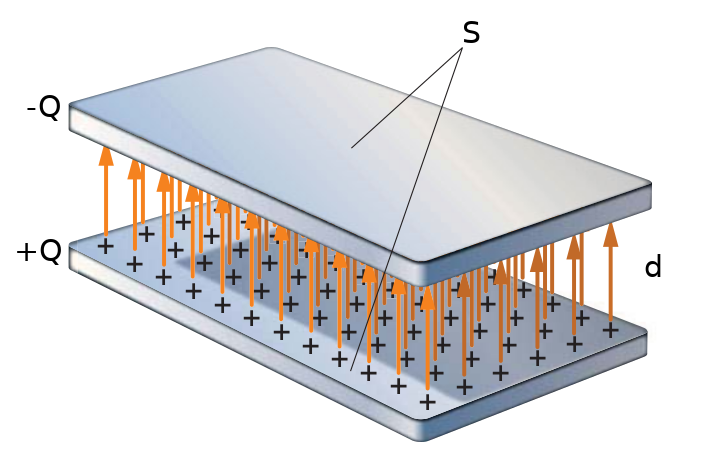
\includegraphics[width=\columnwidth]{img/condensatore.png}
\end{figure}
\end{column}
\begin{column}{0.5\textwidth}
Se le due armature di superficie $ S $ sono separate da una distanza $ d $ (vuota), allora:
\begin{center}
$ \Delta V = Ed = \dfrac{\sigma}{\varepsilon_0} d = \dfrac{Qd}{S\varepsilon_0} $
\end{center}\pause

~

La capacità del condensatore sarà:
\begin{center}
$ C = \dfrac{Q}{\Delta V} = \cancel{Q} \dfrac{S\varepsilon_0}{\cancel{Q}d} $
\end{center}
\end{column}
\end{columns}

\end{frame}

\begin{frame}
\frametitle{Capacità e geometria del condensatore (2)}
\begin{columns}
\begin{column}{0.45\textwidth}
\begin{figure}
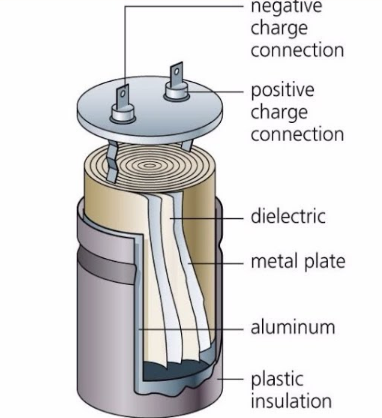
\includegraphics[width=.8\columnwidth]{img/condensatore2.png}
\end{figure}
\end{column}
\begin{column}{0.5\textwidth}
\begin{center}
\colorbox{blue!30}{$ C = \varepsilon_0 \dfrac{S}{d} $}
\end{center}

~

La capacità di un condensatore dipende solo dalle sue dimensioni, dalle sue caratteristiche geometriche: superficie delle armature e distanza tra di esse.
\end{column}
\end{columns}
\end{frame}

\begin{frame}
\frametitle{Esercizio}
\begin{exampleblock}{Elettrone in un un condensatore}
  \small{
  Le armature parallele di un condensatore piano posto nell'aria sono a distanza $ 4,00 \, cm $ l'una dall'altra e hanno area pari a $ 60,0 \, cm^2 $. Sulle armature è presente una carica di $ 5,60 \, nC $. Un elettrone entra nel campo elettrico, attraverso un foro posto nel centro dell'armatura carica positivamente, con velocità di modulo $ v_0 $. Fai l'ipotesi che l'elettrone si muova perpendicolarmente alle armature del condensatore.

  Quale valore deve avere $ v_0 $ perché la velocità dell'elettrone si annulli a metà tra le armature?\hspace*{\fill}[$ 2,72 \times 10^{7} \, m/s $]}
\end{exampleblock}
\end{frame}



\section{Collegamento}


\begin{frame}
\frametitle{Collegamento di condensatori}
\begin{figure}
\ctikzset{bipoles/length=1.0cm}
\begin{circuitikz}[scale=0.4] 
\draw (6,-5) to[capacitor] (10,-5);
\end{circuitikz}
\end{figure}
Spesso nei circuiti incontreremo più condensatori connessi tra loro.
\begin{block}{Capacità equivalente}
Si chiama capacità equivalente $ C_{eq} $ della rete di condensatori quella di un singolo condensatore che, sottoposto alla stessa differenza di potenziale $ \Delta V $ a cui è soggetta l’intera rete, assorbe la stessa carica elettrica.
\begin{center}
$ C_{eq} = \dfrac{Q_{tot}}{\Delta V} $
\end{center}
\end{block}
\end{frame}

\begin{frame}
\frametitle{Collegamento in parallelo}
Nel collegamento in parallelo, le armature dei condensatori sono sottoposte alla stessa differenza di potenziale.
\begin{figure}\centering
\ctikzset{bipoles/length=0.6cm}
\begin{circuitikz}[scale=0.7]
\draw (0,4) to[short] (2,4);
\draw (2,2.5) to[short] (2,5.5);
\draw (2,5.5) to[capacitor=$C_1$] (4,5.5);
\draw (4,5.5) to[short] (4,4);
\draw (2,2.5) to[capacitor=$C_3$] (4,2.5);
\draw (4,2.5) to[short] (4,4);
\draw (4,4) to[short] (6,4);
\draw (2,4) to[capacitor=$C_2$, o-o] (4,4);
\draw [|-|] (0,7) -- (6,7);
\node [above] at (3,7) {$ \Delta V $};
\end{circuitikz}
\end{figure}
\begin{center}
\colorbox{blue!30}{$ C_{eq} = C_1 + C_2 + C_3 + ... $}
\end{center}
\end{frame}





\begin{frame}
\frametitle{Collegamento in serie}
Nel collegamento in serie, ogni armatura porta una carica uguale e contraria a quella dell'armatura immediatamente adiacente.
\begin{figure}\centering
\ctikzset{bipoles/length=1.0cm}
\begin{circuitikz}[scale=0.7]
\draw (0,0) to[capacitor=$C_1$] (2,0);
\draw (2,0) to[capacitor=$C_2$] (4,0);
\draw (4,0) to[capacitor=$C_3$] (6,0);
\draw [|-|] (0,2) -- (6,2);
\node [above] at (3,2) {$ \Delta V $};
\end{circuitikz}
\end{figure}
\begin{center}
\colorbox{blue!30}{$ \dfrac{1}{C_{eq}} = \dfrac{1}{C_1} + \dfrac{1}{C_2} + \dfrac{1}{C_3} + ... $}
\end{center}
\end{frame}

\begin{frame}
\frametitle{Esercizio}
\begin{exampleblock}{Collegamento di condensatori}
  \small{
  Due condensatori hanno capacità $ C_1 = 1,60 \, \mu F $ e $ C_2 = 2,40 \, \mu F $.

  Calcola la capacità equivalente quando i condensatori sono collegati in parallelo.\hspace*{\fill}[$ 4,00 \, \mu F $]
  
  Calcola la capacità equivalente quando i condensatori sono collegati in serie.\hspace*{\fill}[$ 0,960 \, \mu F $]}
\end{exampleblock}
\end{frame}

\section{Energia}

\begin{frame}
\frametitle{Energia immagazzinata}
Per la conservazione dell'energia, l'energia immagazzinata in un condensatore è uguale al lavoro svolto contro le forze elettriche per caricare le sue armature.\pause

~

È possibile dimostrare che il \alert{lavoro di carica} vale:
\begin{center}
\colorbox{blue!30}{$ L = \dfrac{1}{2} QV = \dfrac{1}{2} CV^2 $}
\end{center}

~

I condensatori fungono quindi da ``serbatoi di energia elettrica'' (la bottiglia di Leida del 1745 ne è il primissimo esempio).
\end{frame}


\begin{frame}
\frametitle{Utilizzi dei condensatori}
Oltre che nei circuiti in senso stretto, possiamo trovare i condensatori in altri ambiti della nostra vita.

~

\begin{columns}
\begin{column}{0.3\textwidth}
\visible<1->{\begin{figure}
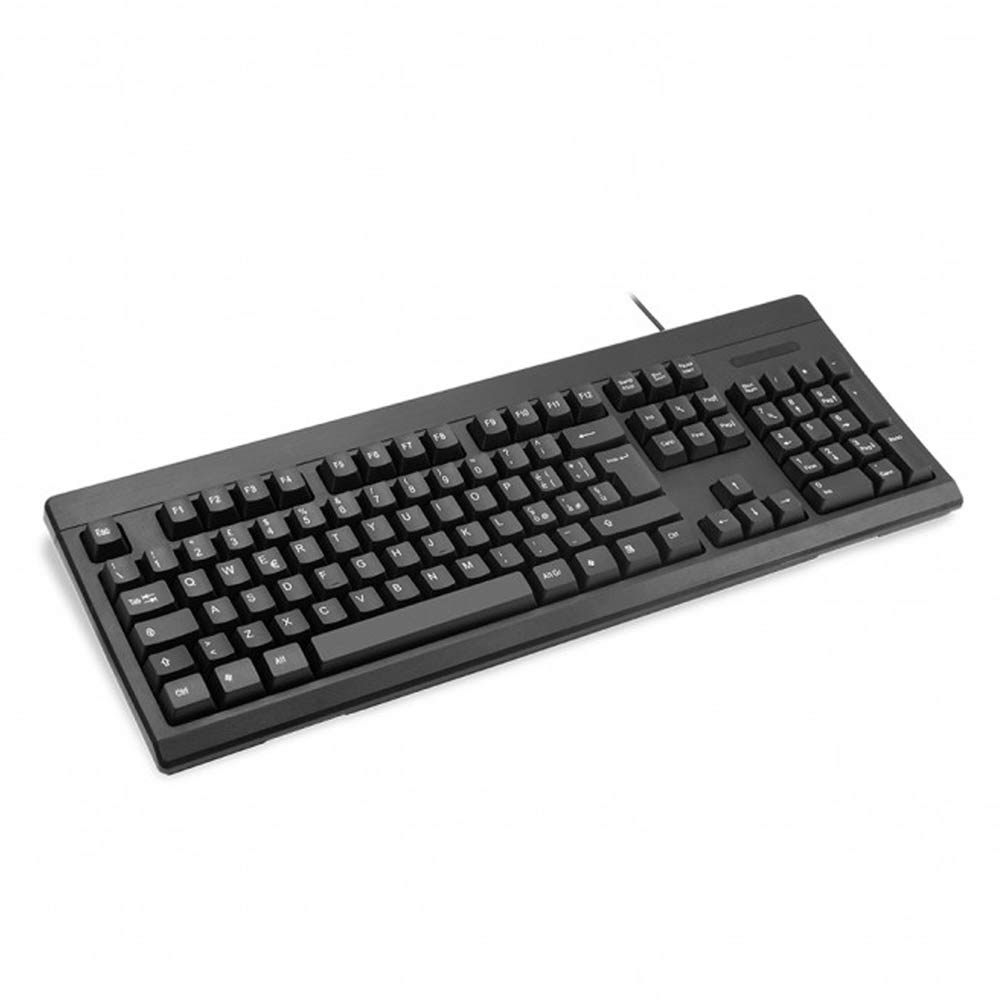
\includegraphics[width=\columnwidth]{img/tastiera.jpg}
\end{figure}}
\end{column}
\begin{column}{0.3\textwidth}
\visible<2->{\begin{figure}
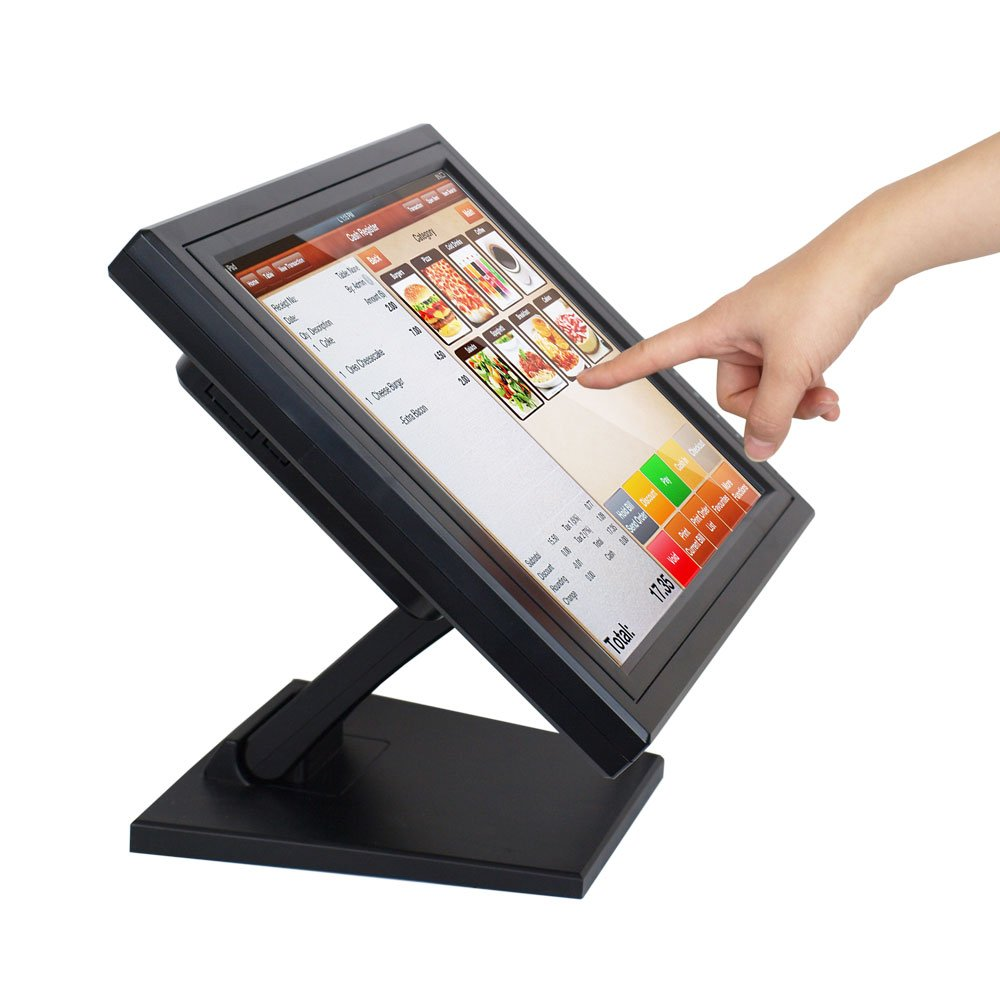
\includegraphics[width=\columnwidth]{img/touchscreen.jpg}
\end{figure}}
\end{column}
\begin{column}{0.3\textwidth}
\visible<3->{\begin{figure}
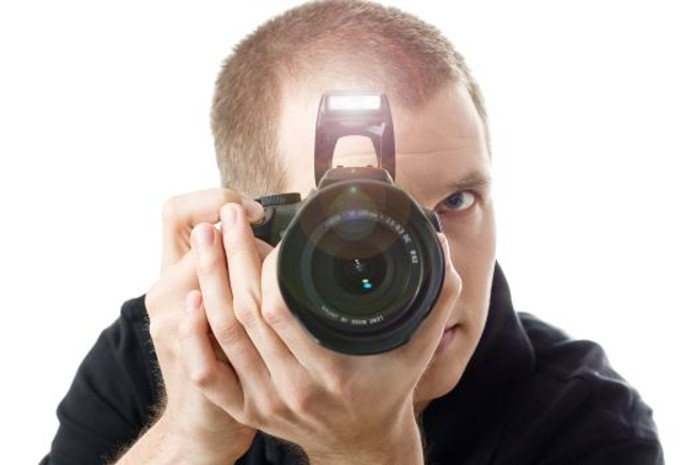
\includegraphics[width=\columnwidth]{img/flash.jpg}
\end{figure}}
\end{column}
\end{columns}
\end{frame}




\end{document}
